\begin{table}[h!]
	\caption{The GradientBoostingClassifier parameters}
	\begin{tabular}{ | l | l | p{7cm} |}
		\hline
		\textbf{Parameter} & \textbf{Default} & \textbf{Description}\\
		\hline
		$n\_estimators$ & 100 & The number of boosting stages to perform. Gradient boosting is fairly robust to over-fitting so a large number usually results in better performance.\\
		\hline
		$learning\_rate$ & 0.1 & learning rate shrinks the contribution of each tree by learning\_rate.\\
		\hline
		$max\_depth$ & 3 & The maximum depth limits the number of nodes in the tree.\\
		\hline
		$min\_samples\_leaf$ & 1 & The minimum number of samples required to be at a leaf node.\\
		\hline
		$max\_features$ & n\_features & The number of features to consider when looking for the best split.\\
		\hline
	\end{tabular}
	\label{table:GBdefaults}
\end{table}
The following set of hyper-parameter values was used:
\begin{itemize}
	\item learning\_rate: [0.1, 0.05, 0.02, 0.01],
	\item max\_depth: [2, 4, 6],
	\item min\_samples\_leaf: [3, 5, 9, 17],
	\item max\_features: [1.0, 0.7, 0.3, 0.1]
\end{itemize}
\subsubsection{Results}
\begin{table}[h!]
	\caption{Grid search output}
	\centering
	\begin{tabular}{ | l | c | c | c | c | c |}
		\hline
		$\bf{params_n}$ & \bf{l\_rate} &  \bf{mx\_depth} & \bf{m\_s\_leaf} & \bf{mx\_features} & \bf{log\_loss} \\ \hline
		$params_1$ & 0.05 & 4 & 17 & 0.7 & 0.6511 \\ \hline
		$params_2$ & 0.10 & 2 & 9 & 0.1 & 0.6756 \\ \hline
		$params_3$ & 0.05 & 4 & 17 & 0.1 & 0.7065 \\ \hline
		$params_4$ & 0.02 & 6 & 5 & 0.3 & 0.7143 \\ \hline
		$params_5$ & 0.05 & 4 & 5 & 0.3 & 0.7226 \\ \hline
	\end{tabular}
\end{table}
\begin{figure}[h!]
    \centering
    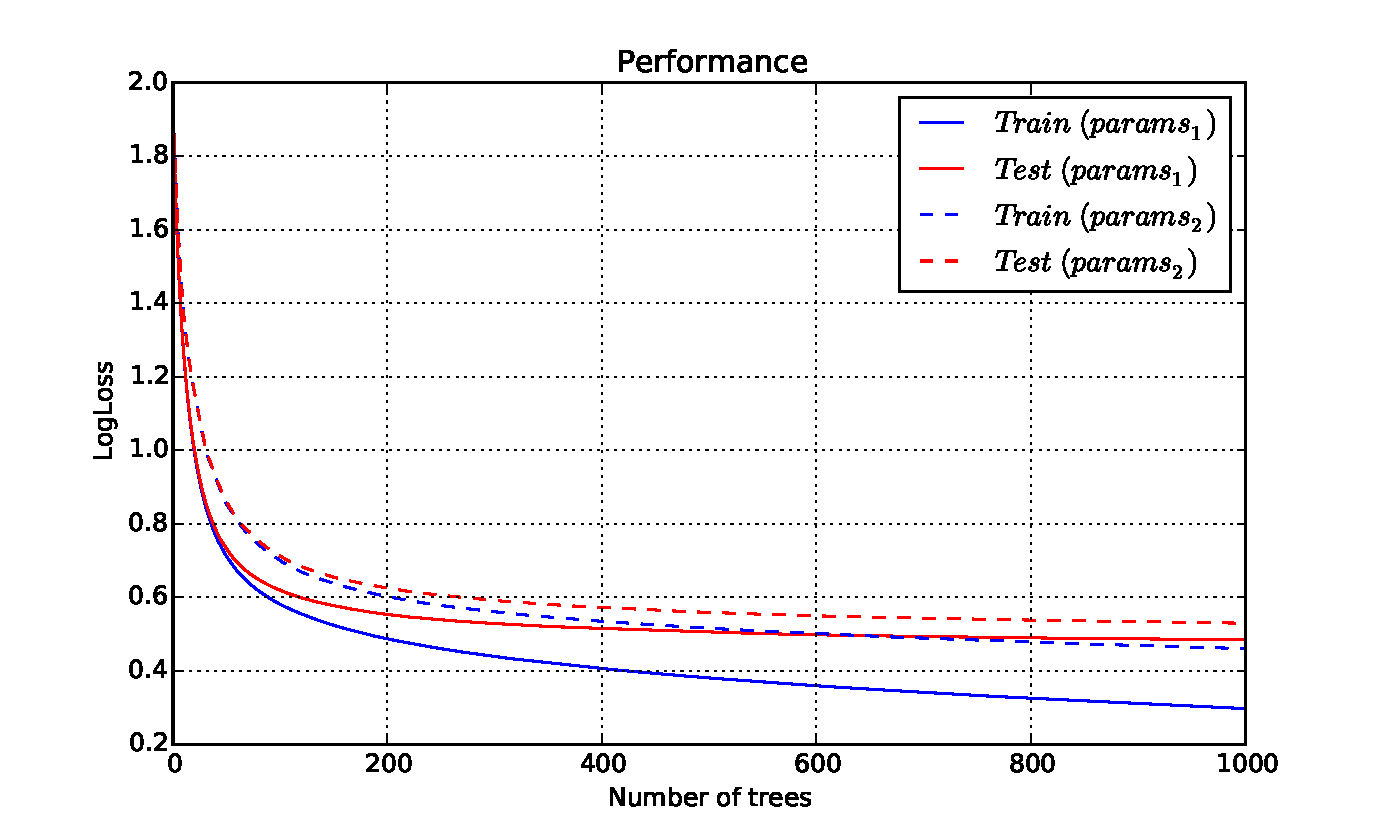
\includegraphics[width=0.86\textwidth]{GBlog_loss}
    \caption{Gradient boosting performance using logarithmic loss as a metric}
    \label{fig:GBlog_loss}
\end{figure}
\begin{figure}[h!]
    \centering
    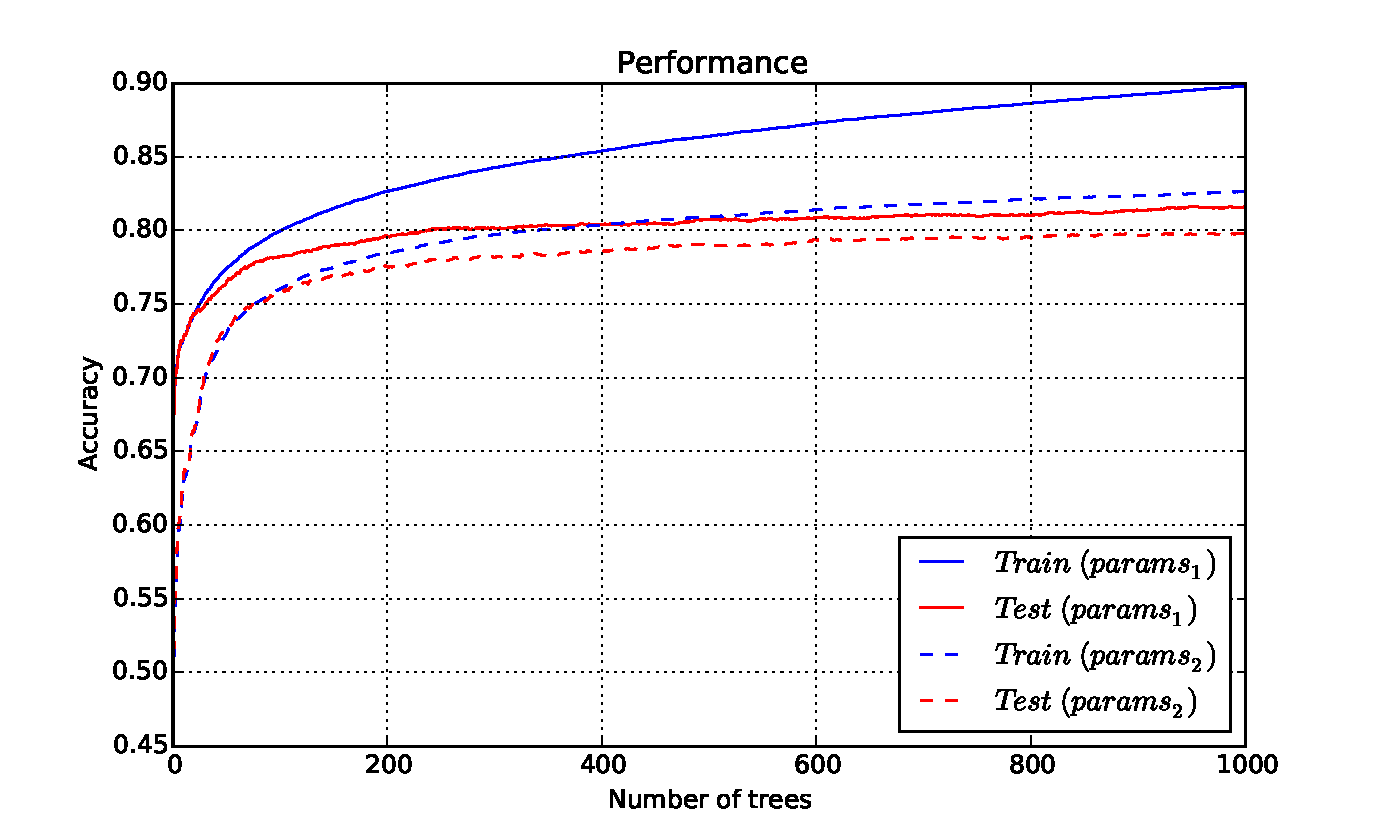
\includegraphics[width=0.9\textwidth]{GBaccuracy}
    \caption{Gradient boosting performance using accuracy as a metric}
    \label{fig:GBaccuracy}
\end{figure}
Knowing that, in boosting algorithms, each new classifier is an expert on the errors of its predecessor, we can compute the performance each time a new tree is added and plot it.

From figure \ref{fig:GBlog_loss} it can be seen that over-fitting is not present even with a large number of tree estimators. Differently from Random Forests, the accuracy changes with each tree that is added due to the fact that each new tree learns the errors of it's predecessor and a better output can be obtained. Performance improvement after the 500th tree is not significant and requires more memory and computation time.

\begin{figure}[h!]
    \centering
    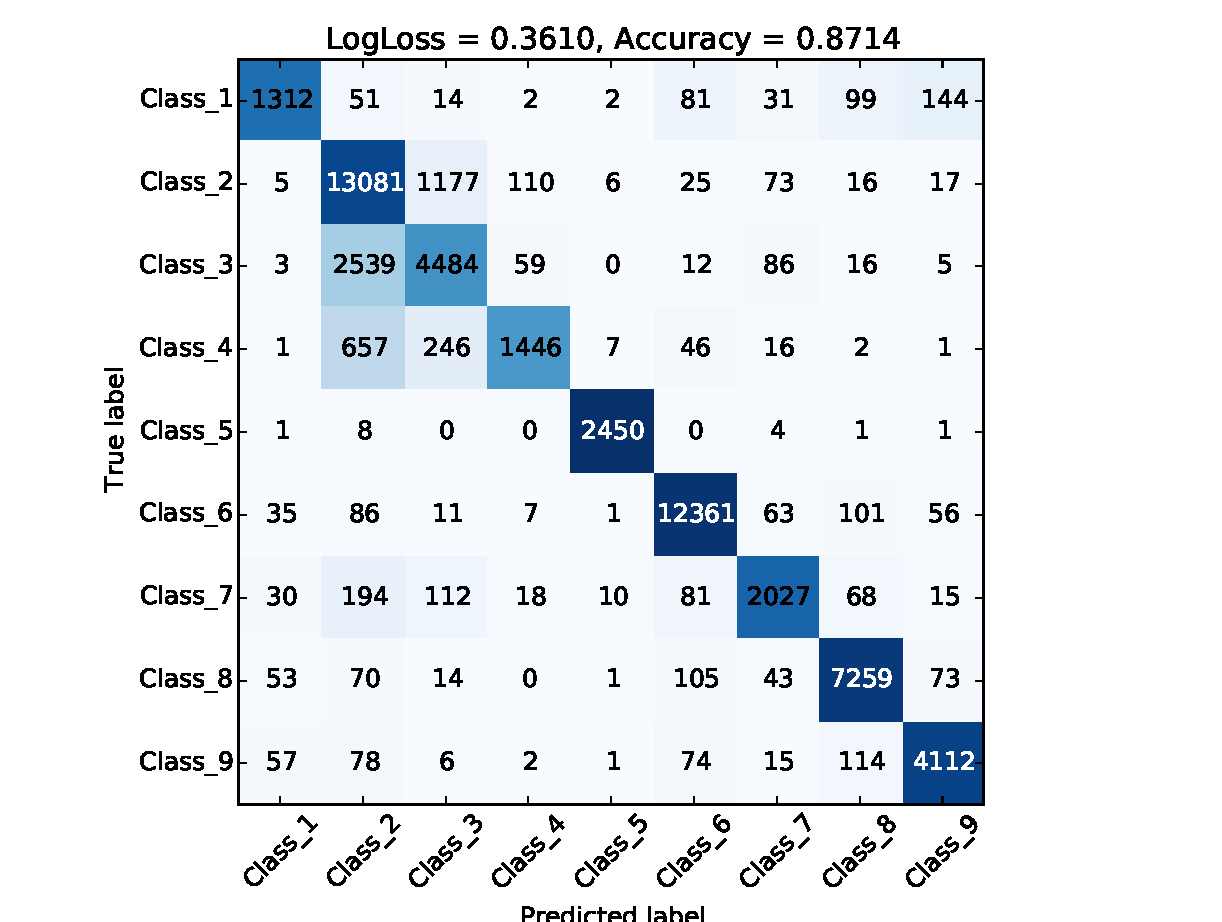
\includegraphics[width=0.69\textwidth]{GBcm_train}
    \caption{Gradient boosting confusion matrix using training set}
    \label{fig:GBcm_train}
\end{figure}
\begin{figure}[h!]
    \centering
    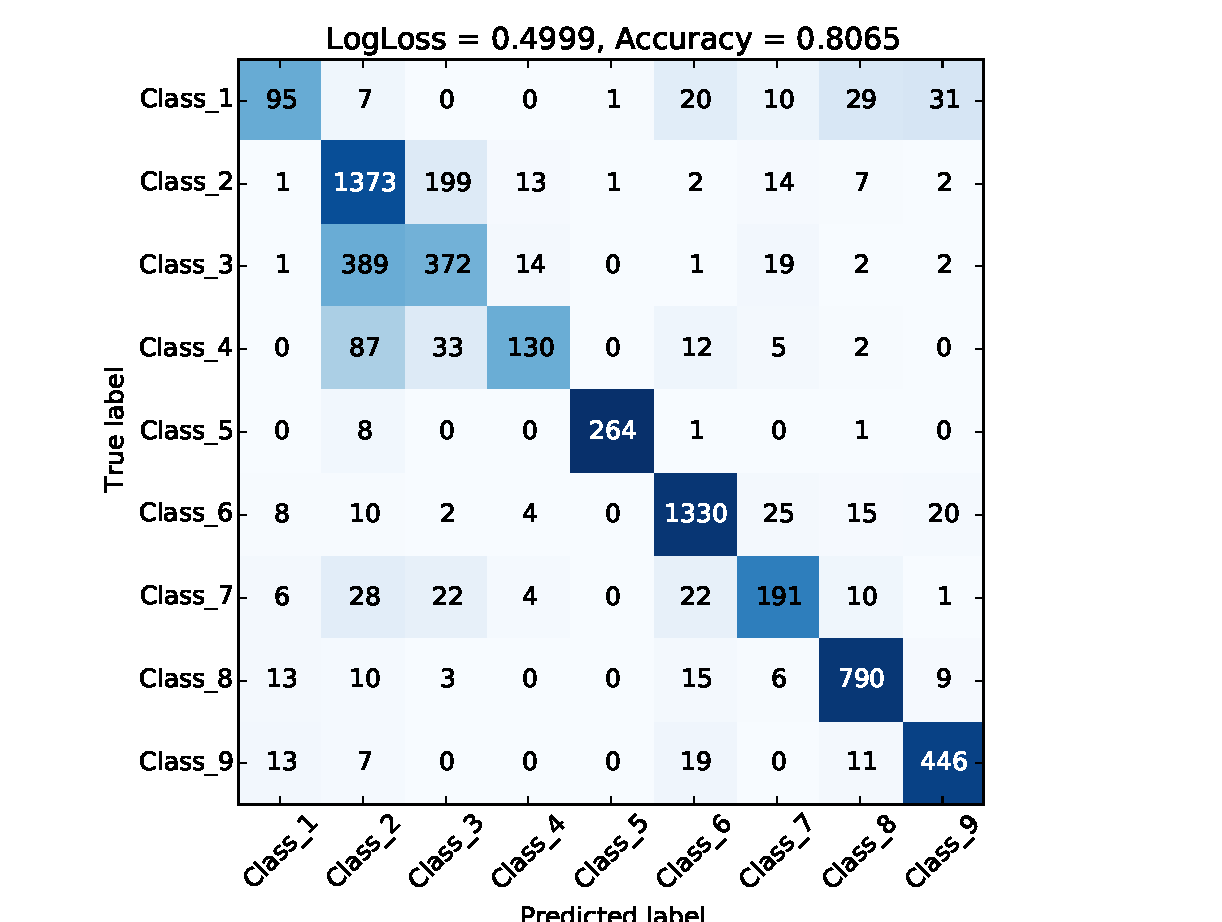
\includegraphics[width=0.7\textwidth]{GBcm_test}
    \caption{Gradient boosting confusion matrix using testing set}
    \label{fig:GBcm_test}
\end{figure}



